\subsection{Gesamtaufbau} \label{sec:gesamtaufbau}
Nachdem nun alle Subsektionen des Prototyps in den vorhergehenden Abschnitten beschrieben wurden, gilt es nun einen gesamtheitlichen Prototypen zu erstellen. Dabei wurden diese, wie in Schema \ref{fig:dojo-schema} zu sehen, zusammengefügt. 

\begin{figure}[H]
	\begin{center}
		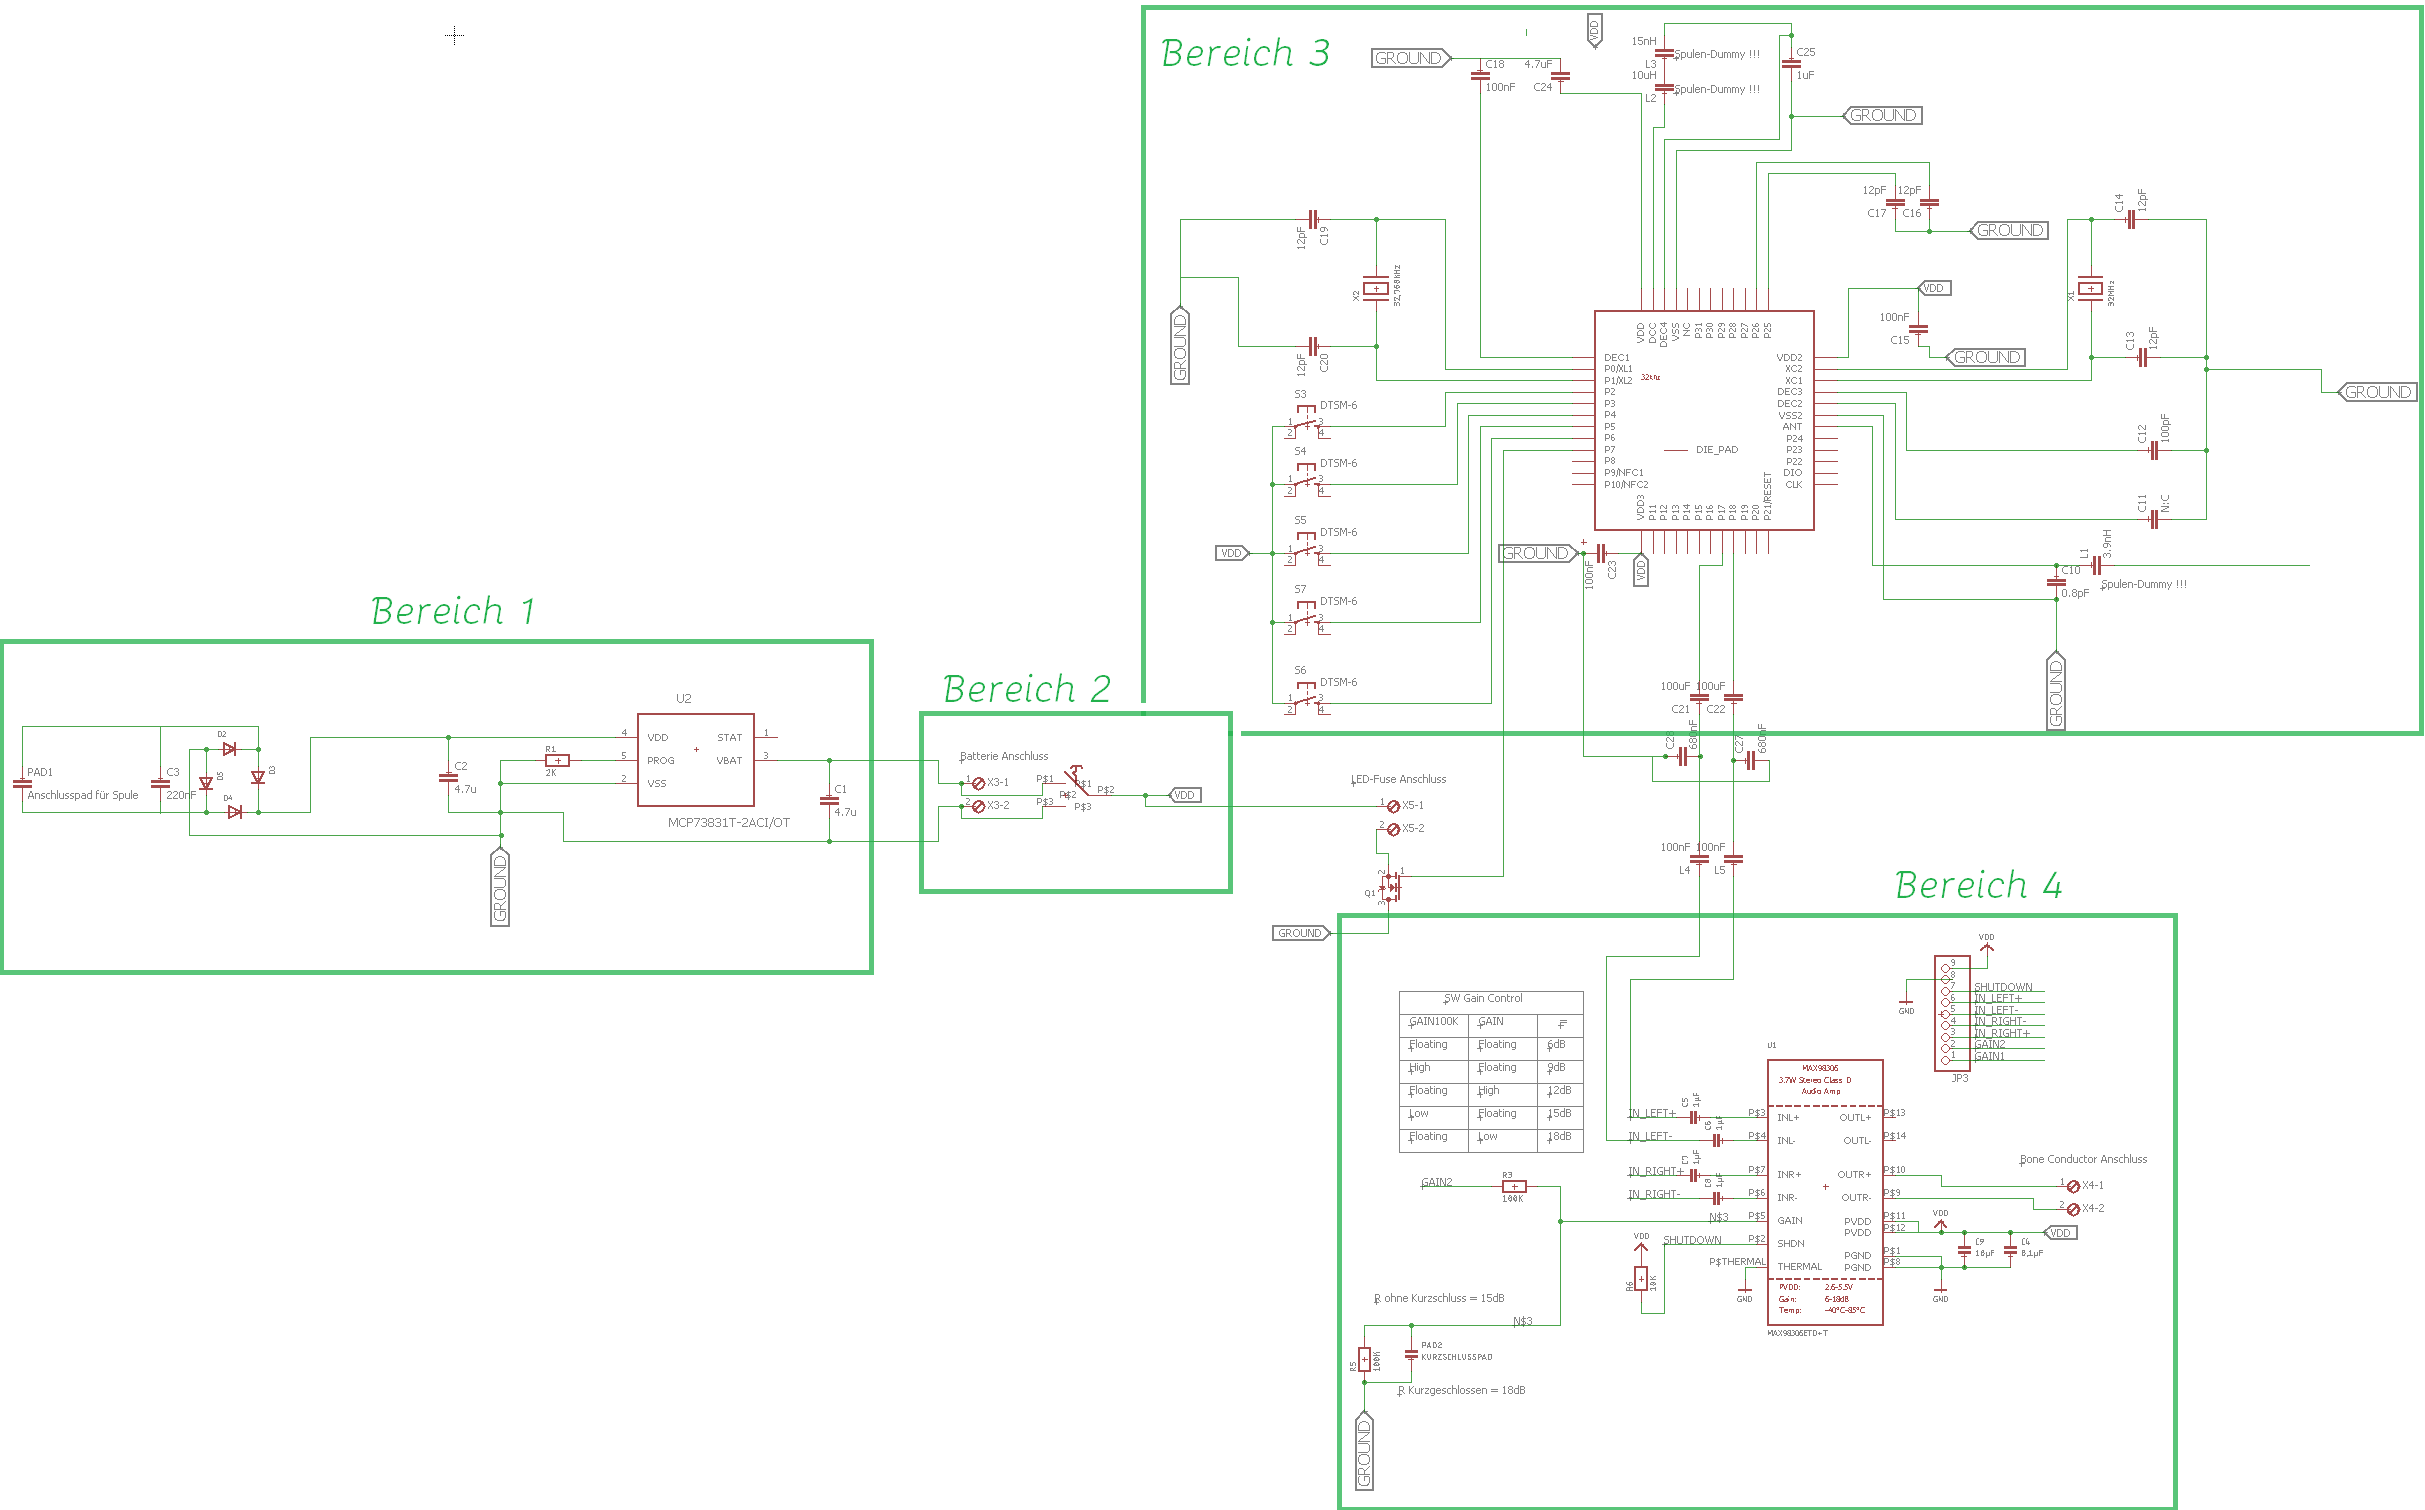
\includegraphics[width=160mm]{data/dojo-schema_2.png}
		\caption[das komplette Schema des Dōjōs]{das komplette Schema des Dōjōs} %picture caption
		\label{fig:dojo-schema}
	\end{center}
\end{figure}


Es ist zu sehen, dass die Ladeschaltung (Bereich 1) mit der Batterie (Bereich 2) verbunden ist und die gesamte Energieversorgung übernimmt. Der Mikrokontroller ist im Bereich 3 ersichtlich und bildet die zentrale Schnittstelle. Der Verstärker und die Audioausgabe sind in Bereich 5 ersichtlich, wobei das Audiofile vor der Ausgabe von einem LC-Filter (Bereich 4) aufbereitet werden muss.
 
In einem weiteren Schritt würde ein Print für in den Dōjō gefertigt. Dieser müsste natürlich wesentlich kleiner sein als dessen Prototyp, damit dieser in den Dōjō hineinpasse. Somit wurde mit dem Layout-Programm Autocad EAGLE ein Layout erstellt, welches fünf Layer besitzt. Die Aussenmasse betragen $17mm$ auf $56mm$ auf $2mm$. Auf dem Top Layer (Layer $1$) wurde die Ladeschaltung und der Verstärker samt Filter platziert. Desweiteren sind die  hardwarespezifische Anschlüsse für die Batterie, den Knochenschallgeber und die Led-Fuseder sowie die fünf Knöpfe ebenfalls auf dem Top Layer. Dies ist damit zu begründen, da diese Subsysteme sehr kleine Ausmasse haben und deshalb effizient platziert werden konnten. Auf dem Bottom Layer (Layer $5$) ist der Komplette Mikrokontroller untergebracht, da dieser aufgrund seiner vielen externen Komponenten mehr Platz benötigt. Desweiteren gilt zu beachten dass bei diesem auf verschiedenste Schematischen Regeln geachtet werden muss, was die Platzierung noch weiter einschrenkte. Auf Layer $3$ wurde die Massefläche untergebracht, damit diese von beiden Aussenlayern gleich weit entfernt ist und somit nicht unnötig lange Masseanschlüsse für einen der beiden Seiten entsteht. Layer $2$ und $4$ dienen als zusätzliche Layer um die Verbindungen der Komponenten auf diesem engen Raum zu ermöglichen. Das finale Layout ist nachfolgend in der Abbildung \ref{fig:Dojo_layout} zu sehen.
\begin{figure}[H]
	\begin{center}
		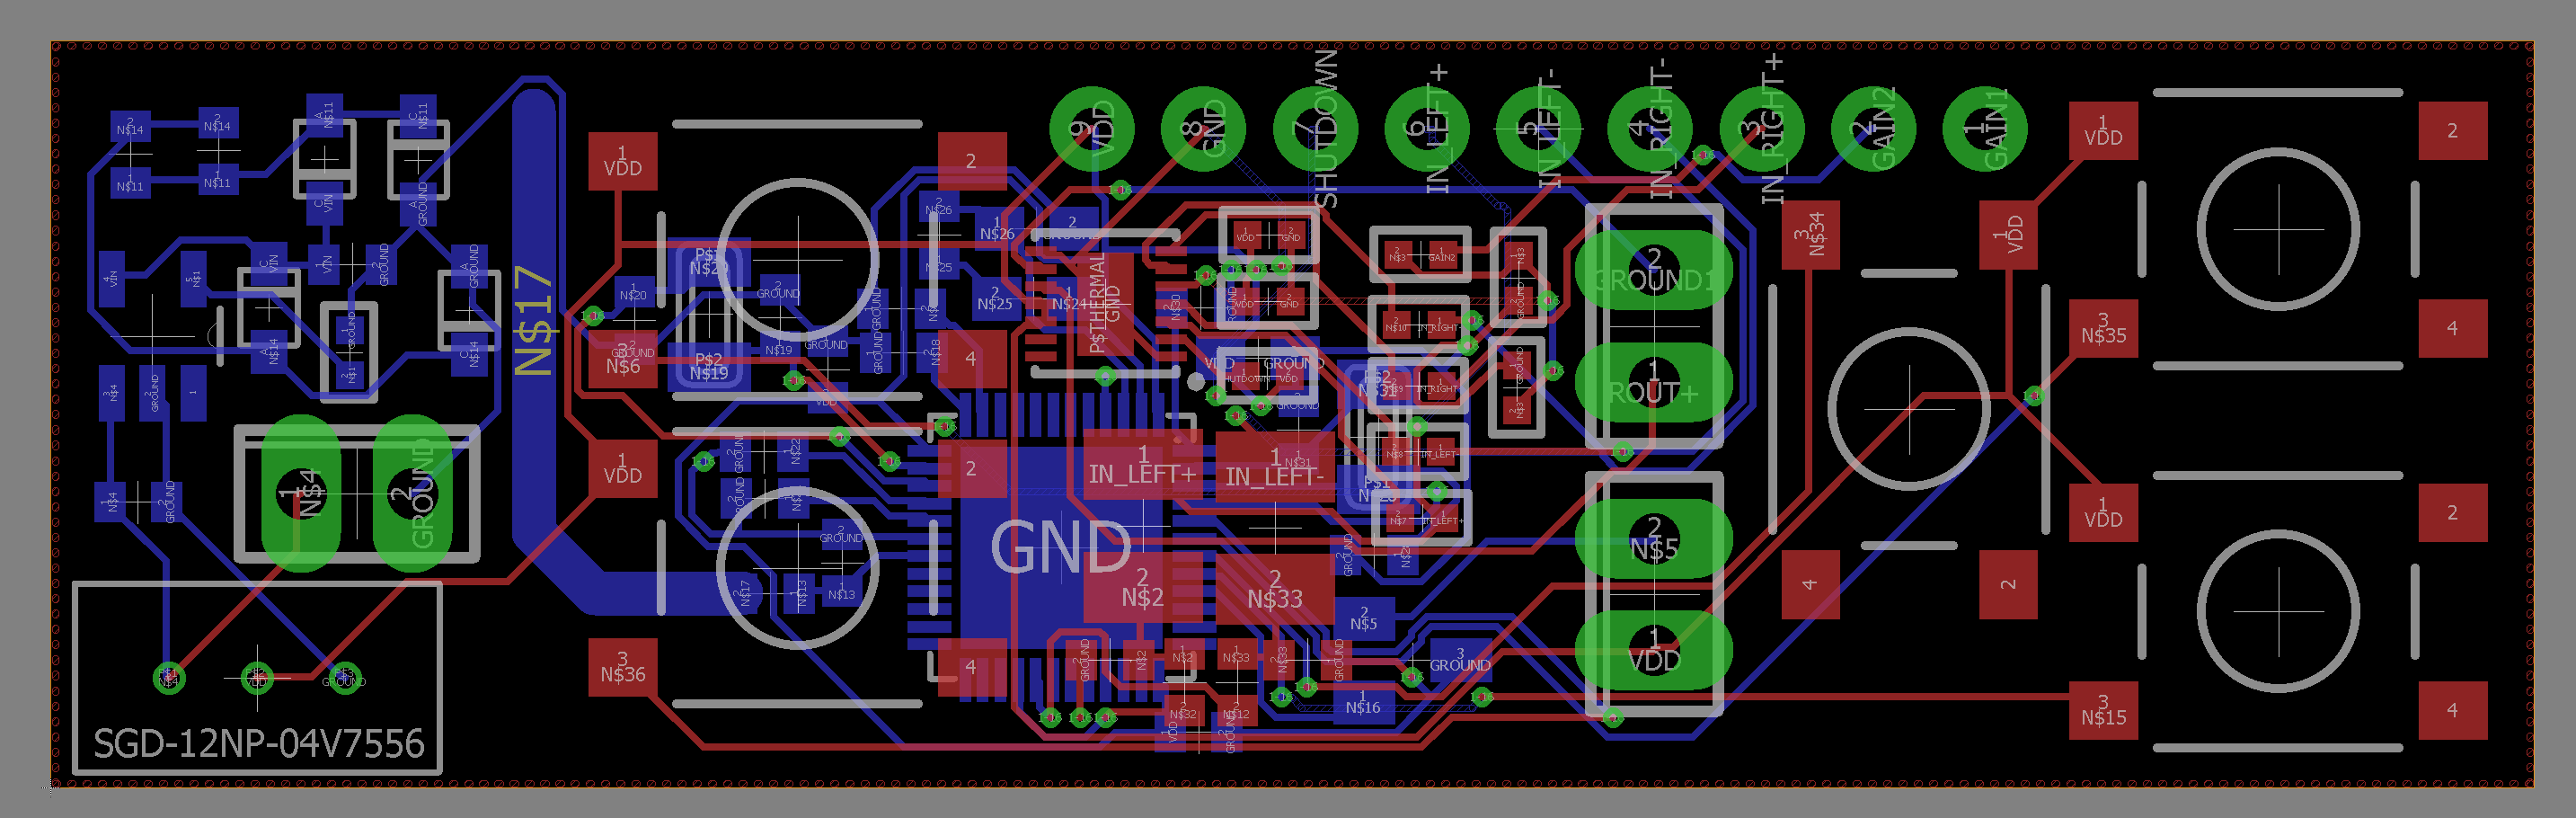
\includegraphics[width=160mm]{data/dojo_layout.png}
		\caption[Das Schema um alle Subsysteme im Dōjō unterzubringen]{Das Schema um alle Subsysteme im Dōjō unterzubringen} %picture caption
		\label{fig:Dojo_layout}
	\end{center}
\end{figure}

Dieser Print wird im innerern des Dōjōs unterhalb des Bedienfeldes eingebaut. Somit können dessen Knöpfe direkt auf die Knöpfe des Printes drücken. Zusätzlich wird seitlich am Dōjō ein kleiner Spalt für den Hauptschalter sein. Dieser ermöglicht zusätzliches Energiesparen wärend der Dōjō nicht gebraucht wird und garantiert zudem ein reibungsloses Laden. Unterhalb des Prints wird die Batterie platziert. Somit liegt das schwerste Bauteil im Dōjō in der Hand des Trägers, was den Schwerpunkt absenkt und so zu einem angenehmeren Tragen beiträgt. Am Boden der Batterie wird die Ladespule befestigt. Da die Batterie lose im inneren des Gehäuses liegt, wirkt diese beim Laden als Anpressgewicht für die Spule.(Da der Dōjō beim Laden aufrecht steht.) Somit ist gewährleistet, dass die Spule immer schön gerade am Boden aufliegt, falls diese durch das herumtragen des Dōjōs verrutscht sein sollte. 
 
Auf der gegenüberliegenden Seite des Dōjōs (also oberhalb des Prints) liegt der Knochenschallsensor. Damit während der Audioübertragung nicht das gesamte Gehäuse vibriert, wird eine Aussparung gemacht. Diese garantiert, dass der vibrierende Teil des Knochenschallsensors unabhängig vom Gehäuse ist und somit direkt auf an den Kopf gehalten werden kann.
 
